%%%%%%%%%%%%%%%%%%%%%%%%%%%%%%%%%%%%%%%%%%%%%%%%%%%%%%%%%%%%%%%%%%%%%%%%%%%%%%%%
% Copyright 2021 Louis Paternault --- http://ababsurdo.fr
%
% Publié sous licence Creative Commons Attribution-ShareAlike 4.0 International (CC BY-SA 4.0)
% http://creativecommons.org/licenses/by-sa/4.0/deed.fr
%%%%%%%%%%%%%%%%%%%%%%%%%%%%%%%%%%%%%%%%%%%%%%%%%%%%%%%%%%%%%%%%%%%%%%%%%%%%%%%%

% Compiler avec lualatex:
%$ lualatex $basename

\documentclass[12pt, tikz]{standalone}

\usetikzlibrary{calc}

\begin{document}

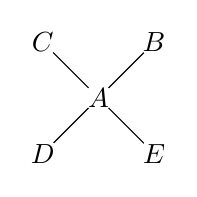
\begin{tikzpicture}
  \tikzstyle{sommet}=[circle, fill=white, minimum size=0em, inner sep=0];

  \coordinate (A) at (0, 0);
  \coordinate (B) at (45:1);
  \coordinate (C) at (135:1);
  \coordinate (D) at (225:1);
  \coordinate (E) at (315:1);

  \foreach \S in {B, C, D, E} {
    \draw (A) -- (\S);
  }
  \draw (A) node[sommet]{$A$};
  \draw (B) node[sommet]{$B$};
  \draw (C) node[sommet]{$C$};
  \draw (D) node[sommet]{$D$};
  \draw (E) node[sommet]{$E$};
\end{tikzpicture}

\end{document}
